\documentclass[a4paper,11pt]{article}
\usepackage{amsmath,amsthm,amsfonts,amssymb,amscd,amstext,vmargin,graphics,graphicx,tabularx,multicol} 
\usepackage[francais]{babel}
\usepackage[utf8]{inputenc}  
\usepackage[T1]{fontenc} 
\usepackage{pstricks-add,tikz,tkz-tab,variations}
\usepackage[autolanguage,np]{numprint} 
\usepackage{xlop}


\setmarginsrb{1.5cm}{0.5cm}{1cm}{0.5cm}{0cm}{0cm}{0cm}{0cm} %Gauche, haut, droite, haut
\newcounter{numexo}
\newcommand{\exo}[1]{\stepcounter{numexo}\noindent{\bf \underline{Exercice~\thenumexo}}}
\reversemarginpar

\opset{decimalsepsymbol={,}}

\newcounter{enumtabi}
\newcounter{enumtaba}
\newcommand{\q}{\stepcounter{enumtabi} \theenumtabi.  }
\newcommand{\qa}{\stepcounter{enumtaba} (\alph{enumtaba}) }
\newcommand{\initq}{\setcounter{enumtabi}{0}}
\newcommand{\initqa}{\setcounter{enumtaba}{0}}

\newcommand\hole[1]{$\bullet$}
\newcommand{\be}{\begin{enumerate}}
\newcommand{\ee}{\end{enumerate}}
\newcommand{\bi}{\begin{itemize}}
\newcommand{\ei}{\end{itemize}}
\newcommand{\bp}{\begin{pspicture*}}
\newcommand{\ep}{\end{pspicture*}}
\newcommand{\bt}{\begin{tabular}}
\newcommand{\et}{\end{tabular}}
\renewcommand{\tabularxcolumn}[1]{>{\centering}m{#1}} %(colonne m{} centrée, au lieu de p par défault) 
\newcommand{\tnl}{\tabularnewline}

\newcommand{\bmul}[1]{\begin{multicols}{#1}}
\newcommand{\emul}{\end{multicols}}

\newcommand{\trait}{\noindent \rule{\linewidth}{0.2mm}}
\newcommand{\hs}[1]{\hspace{#1}}
\newcommand{\vs}[1]{\vspace{#1}}

\newcommand{\N}{\mathbb{N}}
\newcommand{\Z}{\mathbb{Z}}
\newcommand{\R}{\mathbb{R}}
\newcommand{\C}{\mathbb{C}}
\newcommand{\Dcal}{\mathcal{D}}
\newcommand{\Ccal}{\mathcal{C}}
\newcommand{\mc}{\mathcal}

\newcommand{\vect}[1]{\overrightarrow{#1}}
\newcommand{\ds}{\displaystyle}
\newcommand{\eq}{\quad \Leftrightarrow \quad}
\newcommand{\vecti}{\vec{\imath}}
\newcommand{\vectj}{\vec{\jmath}}
\newcommand{\Oij}{(O;\vec{\imath}, \vec{\jmath})}
\newcommand{\OIJ}{(O;I,J)}




\newcommand{\reponse}[1][1]{%
\multido{}{#1}{\makebox[\linewidth]{\rule[0pt]{0pt}{20pt}\dotfill}
}}

\newcommand{\titre}[5] 
% #1: titre #2: haut gauche #3: bas gauche #4: haut droite #5: bas droite
{
\noindent #2 \hfill #4 \\
#3 \hfill #5

\vspace{-1.6cm}

\begin{center}\rule{6cm}{0.5mm}\end{center}
\vspace{0.2cm}
\begin{center}{\large{\textbf{#1}}}\end{center}
\begin{center}\rule{6cm}{0.5mm}\end{center}
}



\begin{document}
\pagestyle{empty}
\titre{Chapitre 3 : Additions et soustractions de nombres décimaux}{}{}{}{}

\vspace*{1cm}

\begin{center}
{\Large \textbf{Niveau 1 :}}
\end{center}

\vspace*{1cm}

$\rightarrow$ \textbf{Vocabulaire sur les additions et soustractions}\\

\vspace*{0.5cm}

\exo \\ Compléter les phrases suivantes.\\


\initqa  \qa La somme de 7 et de 19 est . . . .\\

\qa La différence entre 26 et de 8 est . . . . \\

\qa La somme de . . . . et de 6,5 est  10.\\

\exo \\ Compléter les phrases suivantes.\\


\initqa  \qa La somme de 5,4 et 2,6 est  . . . . \\

\qa La différence entre 7,5 et 0,5 est  . . . . \\

\qa La différence entre 12,5 et . . . . est 8.\\



\vspace*{0.5cm}

$\rightarrow$ \textbf{Additions et soustractions en colonne  }\\

\exo \\ Effectuer les opérations suivantes.\\

\opadd[carryadd=false,resultstyle=\white]{84 321}{578}\kern2cm
\opsub[carrysub=false,resultstyle=\white]{18 743}{6 531}\\

\opadd[carryadd=false,resultstyle=\white]{12,32}{5,04}\kern2cm
\opsub[carrysub=false,resultstyle=\white]{59,76}{28,41}\\

$\rightarrow$ \textbf{Calculs en ligne  }\\

\exo \\ Calculer les sommes suivantes en effectuant des regroupements astucieux.\\

\initqa \qa 15 + 34 + 45 + 46 = 15 + . . . + 34 + . . .\\
= . . . . . . . . . . . . \\



\qa 127 + 34 + 33 + 106 = 127 + . . . + 34 + . . .\\
= . . . . . . . . . . . . \\

\exo \\ Calculer les sommes suivantes en effectuant des regroupements astucieux.\\

\initqa \qa 32 + 65 + 18 + 15 = 32 + . . . + 65 + . . .\\
= . . . . . . . . . . . . \\



\qa 150 + 123 + 350 + 377 + 12 = 150 + . . . + 123 + . . . + 12\\
= . . . . . . . . . . . . \\

$\rightarrow$ \textbf{Calcul mental}\\


\exo \\ Effectuer les calculs ci-dessous.\\

\initqa \qa 37 + 109 = . . . .\\

\qa 67 + 15 = . . . .\\

\qa 23 - 9 = . . . .\\

\qa 328 - 11 = . . . .\\

\exo \\ Compléter par le nombre qui convient.\\

\initqa \qa  . . . - 11 = 67\\

\qa . . . - 9 = 23\\

\qa 6,7 + . . . = 10,3\\

\qa  . . . + 74,1 = 100\\

\exo \\ Entourer le meilleur ordre de grandeur du résultat de chaque calcul.\\

\begin{tabular}{|c|p{2cm}|p{2cm}|p{2cm}|}
\hline 
Calcul & \multicolumn{3}{c|}{Ordre de grandeur du résultat} \\ 
\hline 
38,45 + 19,87 & 40 & 50 & 60 \\ 
\hline 
57,83 - 28,79 & 90 & 40 & 30 \\ 
\hline 
\end{tabular} 

\vspace*{0.2cm}

\exo \\ Retrouver parmi les 4 propositions le bon résultat.\\

\begin{tabular}{|c|c|c|c|c|}
\hline 
Calcul & \multicolumn{4}{c|}{Résultats possibles} \\ 
\hline 
975 + 315 =  & 1 290  & 1 130 & 1 291 & 1 560 \\ 
\hline 
7 147 + 2 067 = & 9 103 & 8 734 & 9 214 & 9 315 \\ 
\hline 
601 657 - 304 = & 600 353  & 601 353  & 601 358 & 601 347 \\ 
\hline 
\end{tabular} 

\vspace*{0.2cm}



$\rightarrow$ \textbf{Problèmes (guidés ou non)}\\

\exo \\ Au retour des vacances, la valise de Samuel pèse 19,6 kg. Une fois qu'il en a sorti les cadeaux pour sa famille, elle pèse 11,9 kg.\\
Calculer la masse des cadeaux ramenée par Samuel.\\

Calculs en ligne :\\
\reponse[2]\\

Phrase réponse :\\
Samuel a ramené . . . . kg de cadeaux pour sa famille.\\

\exo \\ Le père d'Agathe a 37 années de plus que sa fille et, aujourd'hui, il fête ses 49 ans.\\
Quel est l'âge d'Agathe ?\\

Calculs en ligne :\\
\reponse[2]\\

Phrase réponse :\\
Agathe a . . . ans.\\

\exo \\ Laura part faire de la randonnée en Haute-Savoie, dans le massif des 
Bauges. Son altitude de départ est de 928 m. Elle atteint le plus haut sommet, l'Arcalod, après avoir gravi un dénivelé de 1289 m.\\
Quelle est l'altitude de l'Arcalod ?\\

Calculs en ligne :\\
\reponse[2]\\

Phrase réponse :\\
Le sommet de l'Arcalod est à . . . . . m d'altitude.\\

\exo \\ Pour chaque problème, écrire l'opération qu'il faut effectuer pour le résoudre. Aucun résultat n'est demandé.\\

\begin{tabular}{|p{12cm}|p{5cm}|}
\hline 
\textbf{Énoncés} & \textbf{Opération pour résoudre le problème} \\ 
\hline 
Paul parcourt 420 m pour passer prendre son ami Léo puis 630 m pour se rendre au collège. Quelle distance parcourt-il ? &  \\ 
\hline 
Max pèse 36 kg.Il monte sur une balance avec son chien et lit 42,7 kg. Combien pèse son chien ? &  \\ 
\hline 
Julie, âgée de 14 ans, a 7 ans de moins de Maxime. Quel âge a Maxime ? &  \\ 
\hline 
A un jeu, Théo a marqué 4 500 points, soit 750 de plus que Raphaêl. Quel est le score de Raphaêl ? &  \\ 
\hline 
\end{tabular} 

\vspace*{0.3cm}


$\rightarrow$ \textbf{Notion de durée}\\

\exo \\ Compléter les calculs et les conversions.\\

\initqa \qa 4h = . . . . min\\

\qa 180 s = . . . . min\\

\qa 3 jours = . . . . h\\

\qa 48 h = . . . . jours\\

\qa 120 min = . . . . h\\


\exo \\ Effectuer les calculs suivants.\\

\initqa \qa 3 h 10 min - 2 h 10 min = . . . . .\\

\qa 3 h 18 min + 1 h 42 min = . . . . .\\

\qa 2 h 38 min + 1 h 22 min = . . . . .\\

\qa 4 h 15 min - 1h 15 min = . . . . .\\

\begin{center}
{\Large \textbf{Niveau 2 :}}
\end{center}

\vspace*{1cm}

$\rightarrow$ \textbf{Vocabulaire sur les additions et soustractions}\\

\vspace*{0.5cm}

\exo \\ On sait que 7 + 4 = 11 et  23 - 8 = 15.\\
En utilisant les bons mots de vocabulaire, compléter les phrases suivantes.\\

\initqa \q \qa 11 est  la . . . . . . . . . . . de 4 et de 7.\\

\qa 7 et 4 sont les . . . . . . . . . . . . de la . . . . . . . . . . . . .\\

\q \initqa \qa 15 est la . . . . . . . . . . . . . de 23 et de 8.\\

\qa 23 et 8 sont les . . . . . . . . . . . . . . de la . . . . . . . . . . . . . \\




\vspace*{0.5cm}

$\rightarrow$ \textbf{Additions et soustractions en colonne  }\\

\exo  \\ Effectuer les opérations suivantes.\\

\opadd[carryadd=false,resultstyle=\white]{85,25}{32,18}\kern2cm
\opsub[carrysub=false,resultstyle=\white]{125,8}{45,6}\\

\opadd[carryadd=false,resultstyle=\white]{58 630,07}{105 982,631}\kern2cm
\opsub[carrysub=false,resultstyle=\white]{3 514}{1 052,3}\\


$\rightarrow$ \textbf{Calculs en ligne  }\\

\exo \\ Calculer les sommes suivantes en effectuant des regroupements astucieux.\\

\initqa \qa 8,5 + 12,7 + 1,5 = 8,5 + . . . + 12,7\\
= . . . . . . . . . . . . \\



\qa 32 + 3,5 + 28 + 6,5 = 32 + . . . + 3,5 + . . . \\
= . . . . . . . . . . . . \\

\exo \\ Calculer les sommes suivantes en effectuant des regroupements astucieux.\\

\initqa \qa 8,5 + 43 + 6,5 + 57 = 8,5 + . . . + 43 + . . . \\
= . . . . . . . . . . . . \\



\qa 3,5 + 113 + 37 + 5,5 = 3,5 + . . . + 113 + . . . \\
= . . . . . . . . . . . . \\


\exo \\ Calculer les sommes suivantes en effectuant des regroupements astucieux.\\

\initqa \qa 10,5 + 23 + 17 + 8,5 = 10,5 + . . . + 23 + . . . \\
= . . . . . . . . . . . . \\



\qa 192 + 0,5 + 6,5 + 8 + 36 = 192 + . . . + 0,5 + . . . +36 \\
= . . . . . . . . . . . . \\

\exo \\ Calculer les sommes suivantes en effectuant des regroupements astucieux.\\

\initqa \qa 9,5 + 14 + 97 + 0,5 + 3 + 46 = 9,5 + . . . + 14 + . . . + 97 + . . . \\
= . . . . . . . . . . . . \\



\qa 105,5 + 1 032 + 94,5 + 68 + 7 = 105,5 + . . . + 1 032 + . . . + 7 \\
= . . . . . . . . . . . . \\

$\rightarrow$ \textbf{Calcul mental}\\


\exo \\ Effectuer les calculs ci-dessous.\\

\initqa \qa 29,7 - 9,3 = . . . .\\

\qa 128 + 432 = . . . .\\

\qa 4,57 + 1,083 = . . . .\\

\qa 26 - 1,2 = . . . .\\

\exo \\ Compléter par le nombre qui convient.\\

\initqa \qa  358 + . . . = 1 000\\

\qa . . . + 741 = 1 000\\

\qa 45,1 - . . . = 10,9\\

\qa  . . . - 8,7 = 4,6\\

\exo \\ Entourer le meilleur ordre de grandeur du résultat de chaque calcul.\\

\begin{tabular}{|c|p{2cm}|p{2cm}|p{2cm}|}
\hline 
Calcul & \multicolumn{3}{c|}{Ordre de grandeur du résultat} \\ 
\hline 
12 107 + 4 892 & 15 000 & 16 000 & 17 000 \\ 
\hline 
1 315,4 - 231,9 & 1 500 & 1 100 & 1 000 \\ 
\hline 
\end{tabular} 

\vspace*{0.2cm}

\exo \\ Retrouver parmi les 4 propositions le bon résultat.\\

\begin{tabular}{|c|c|c|c|c|}
\hline 
Calcul & \multicolumn{4}{c|}{Résultats possibles} \\ 
\hline 
6,345 + 2,971  =  & 9,36 & 9,316 & 8,316 & 9,786 \\ 
\hline 
7 147 - 2 067 = & 9 655 & 6 805 & 5 085 & 5 803 \\ 
\hline 
74,264 – 37,764 = & 36,5  & 36,9426 & 75,5 & 36,841 \\ 
\hline 
\end{tabular} 

\vspace*{0.2cm}

\exo \\ Dans ce tableau, les sommes des nombres doivent toujours être égales sur chaque ligne, chaque colonne et chaque diagonale.

\begin{center}
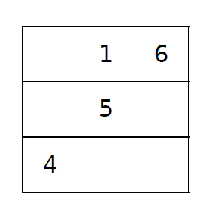
\includegraphics[scale=0.8]{carre.eps} 
\end{center}

$\rightarrow$ \textbf{Problèmes (guidés ou non)}\\

\exo \\Déborah a 25,60 euros. Sa grand-mère lui donne 45,40 euros.\\
 Combien Déborah a-t-elle d'argent ? \\

Calculs en ligne :\\
\reponse[2]\\

Phrase réponse :\\
Déborah possède . . . . euros.\\

\exo \\ Voici un tableau qui regroupe les achats de Mai au supermarché. \\
Quel est le montant total dépensé pour ses courses ?\\

\begin{tabular}{|c|c|}
\hline 
Article & Prix (en euros) \\ 
\hline 
Courgettes & 1,60 \\ 
\hline 
Tomates & 2,40 \\ 
\hline 
Tomme de chèvre & 10,25 \\ 
\hline 
Pack d'eau & 5,75 \\ 
\hline 
Thon & 4 \\ 
\hline 
Farine & 1,25 \\ 
\hline 
\end{tabular} 

Calculs en ligne :\\
\reponse[2]\\

Phrase réponse :\\
Mia a dépensé . . . . euros pour ses courses.\\

\exo \\ Lors d'une épreuve de ski de fond de 2,5 km de long, Martin apprend qu'il a encore 1,775 km à parcourir.\\
Quelle distance a-t-il déjà parcouru ?\\

Calculs en ligne :\\
\reponse[2]\\

Phrase réponse :\\
Martin a déjà parcouru . . . . km.\\

\exo \\ Un ostréiculteur vend 96,5 kg d'huîtres à un restaurateur puis 67,85 kg à un autre et enfin 227 kg à un troisième.\\
Quelle masse d'huîtres a-t-il vendu?\\

Calculs en ligne :\\
\reponse[2]\\

Phrase réponse :\\
L'ostréiculteur a vendu . . . . kg d'huîtres.\\

\vspace*{0.3cm}

$\rightarrow$ \textbf{Notion de durée}\\

\exo \\ Compléter les calculs et les conversions.\\

\initqa \qa 1 h = . . . . s\\

\qa 360 min = . . . . h\\

\qa 3 h  = . . . . min\\

\qa 180 s = . . . . min\\

\qa 72 min = . . . . h . . . . min\\


\exo \\ Effectuer les calculs suivants.\\

\initqa \qa 3 h 15 min + 20 min = . . . . .\\

\qa 2 h 35 min + 3 h 25 min = . . . . .\\

\qa 5 h 28 min - 4 h 11 min = . . . . .\\

\qa 1 h - 38 min = . . . . .\\












\begin{center}
{\Large \textbf{Niveau 3 :}}
\end{center}

\vspace*{1cm}

$\rightarrow$ \textbf{Vocabulaire sur les additions et soustractions}\\

\vspace*{0.5cm}

\exo \\ Compléter les phrases suivantes.\\


\initqa  \qa La somme de 104,67 et 82,36 est  . . . . \\

\qa La différence entre 56,78 et 34,21 est  . . . . \\

\qa La différence entre 1 012 et . . . . est 33,61.\\

\exo \\ La somme de deux nombres est 78,92. Un des deux nombres est 29,6.\\ Quel est le second nombre ?\\


\vspace*{0.5cm}


$\rightarrow$ \textbf{Additions et soustractions en colonne  }\\

\exo \\  Effectuer les opérations suivantes.\\

\includegraphics[scale=0.5]{operation1.eps} \\

\opsub[carrysub=false,resultstyle=\white]{135,8}{6,13}\kern2cm
\opsub[carrysub=false,resultstyle=\white]{90 123,081}{7 654,903}\\


\exo \\ par les chiffres qui conviennent.\\


\opadd[carryadd=false,operandstyle.1=\hole]{1256}{9861} \hspace*{2cm} \opadd[carryadd=false,operandstyle.1.1=\hole,operandstyle.1.2=\hole,operandstyle.1.3=\hole,operandstyle.1.-1=\hole,operandstyle.1.-2=\hole]{893,40}{29,52}\\



\exo \\ Compléter par les chiffres qui conviennent.\\


\opadd[carryadd=false,operandstyle.2.1=\hole,operandstyle.2.2=\hole,resultstyle.4=\hole,resultstyle.3=\hole]{3456}{725} \hspace*{2cm} \opadd[carryadd=false,operandstyle.1.1=\hole,operandstyle.1.2=\hole,operandstyle.1.-1=\hole,operandstyle.1.-2=\hole]{55,98}{39,2}\\



$\rightarrow$ \textbf{Calculs en ligne  }\\

\exo \\ Calculer les sommes suivantes en effectuant des regroupements astucieux.\\

\initqa \qa 17 + 5,35 + 53 + 14,65  = 17 + . . . + 5,35 + . . . \\
= . . . . . . . . . . . . \\



\qa 109,25 + 74 + 1,75 = 109,25 + . . . + 74 \\
= . . . . . . . . . . . . \\






\exo \\ Calculer les sommes suivantes en effectuant des regroupements astucieux.\\

\initqa \qa 13,5 + 12,9 + 2,1 + 1,5  = 13,5 + . . . + 12,9 + . . . \\
= . . . . . . . . . . . . \\



\qa 7,25 + 6,1 + 5,75 + 3,9 = 7,25 + . . . + 6,1 + . . . \\
= . . . . . . . . . . . . \\



\exo \\ Calculer les sommes suivantes en effectuant des regroupements astucieux.\\

\initqa \qa 3,4 + 13,7 + 8,6 + 10,3 + 24  = 3,4 + . . . + 13,7 + . . . + . . . \\
= . . . . . . . . . . . . \\



\qa 12,1 + 12,4 + 12,9 + 12,6 = 12,1 + . . . + 12,4 + . . . \\
= . . . . . . . . . . . . \\

\exo \\ Calculer les sommes suivantes en effectuant des regroupements astucieux.\\

\initqa \qa 1 036 + 21,4 + 14 + 9,3  = 1 036 + . . . + 21,4 + . . . + . . . \\
= . . . . . . . . . . . . \\



\qa 3,6 + 122 + 2,4 + 25 + 178 = 3,6 + . . . + 122 + . . .  + 25\\
= . . . . . . . . . . . . \\

\exo \\ Calculer les sommes suivantes en effectuant des regroupements astucieux.\\

\initqa \qa 2,1 + 5,3 + 3 + 1,9 + 10,7  = 2,1 + . . . + 5,3 + . . . + . . . \\
= . . . . . . . . . . . . \\



\qa 6,8 + 5,7 + 4,3 + 3,2 + 103 = 6,8 + . . . + 5,7 + . . . + . . . \\
= . . . . . . . . . . . . \\

\vspace*{0.5cm}

$\rightarrow$ \textbf{Calcul mental}\\


\exo \\ Effectuer les calculs ci-dessous.\\

\initqa \qa 12,4 + 11,25 = . . . .\\

\qa 72,5 - 9 = . . . .\\

\qa 33,7 + 19,03 = . . . .\\

\qa 13,3 - 6,21 = . . . .\\

\exo \\ Compléter par le nombre qui convient.\\

\initqa \qa  2,51 + . . . = 6\\

\qa . . . + 40,8 = 45,6\\

\qa 27,5 - . . . = 13,2\\

\qa  . . . - 13 = 77,12\\

\exo \\ Entourer le meilleur ordre de grandeur du résultat de chaque calcul.\\

\begin{tabular}{|c|p{2cm}|p{2cm}|p{2cm}|}
\hline 
Calcul & \multicolumn{3}{c|}{Ordre de grandeur du résultat} \\ 
\hline 
496,89 + 1 001,25 + 199,67 & 1 400 & 1 500 & 1 550 \\ 
\hline 
2 003,582 - 998,75 - 49,85 & 1 800 & 1 850 & 1 900 \\ 
\hline 
\end{tabular} 

\vspace*{0.5cm}

\exo \\ Compléter le tableau suivant comme dans l'exemple.\\

\begin{tabular}{|c|c|c|c|}
\hline 
x & y & x + y & x - y \\ 
\hline 
6 & 1,5 & 6 + 1,5 = 7,5 & 6 - 1,5 = 4,5 \\ 
\hline 
16,3 & 6,5 &  &  \\ 
\hline 
104,47 & 65,1 &  &  \\ 
\hline 
12,9 &  & 21,6 &  \\ 
\hline 
\end{tabular} 

\vspace*{0.5cm}

\exo \\ Dans ce tableau, les sommes des nombres doivent toujours être égales sur chaque ligne, chaque colonne et chaque diagonale.\\

\begin{center}
\begin{tabular}{|c|c|c|}
\hline 
 &  & 7,5 \\ 
\hline 
 & 4,5 & 2,5 \\ 
\hline 
1,5 &  &  \\ 
\hline 
\end{tabular} 
\end{center}

\exo \\ Compléter chaque case par la somme des nombres qui figurent dans les deux cases situées juste en dessous. \\

\textbf{Exemple :} \includegraphics[scale=0.65]{pyramide2.eps} \\

\includegraphics[scale=0.65]{pyramide1.eps}\\

$\rightarrow$ \textbf{Problèmes (guidés ou non)}\\

\exo \\ L'Algérie a 6 343 km de frontières terrestres :\\
1 559 km partagés avec le Maroc, 1376 km avec le Mali, 982 km avec la Libye, 965 km avec la Tunisie, 956 km avec le Niger, 463 km avec la Mauritanie et le reste avec le Sahara Occidental.\\
Combien de kilomètres de frontières séparent l'Algérie et le Sahara Occidental ?\\

Calculs en ligne :\\
\reponse[2]\\

Phrase réponse :\\
\reponse[1]\\



\exo \\ La Guyane Française fait partie du plateau des 5 Guyanes. C'est le plus grand département français.\\

\begin{tabular}{|c|c|}
\hline 
Les 5 Guyanes & Superficie (en $km^{2}$) \\ 
\hline 
Guyana & 214 970 \\ 
\hline 
Guyane Française &  \\ 
\hline 
Nord du Brésil & 62 000 \\ 
\hline 
Sud-est du Venezuela & 415 000 \\ 
\hline 
Suriname & 163 265 \\ 
\hline 
Total & 939 085 \\ 
\hline 
\end{tabular} 

\vspace*{0.2cm}

Quelle est sa superficie ?\\



Calculs en ligne :\\
\reponse[2]\\

Phrase réponse :\\
\reponse[1]\\

\exo \\ Erwan se rend en voiture de Brest à Bayonne. Quelle distance parcourt-il ?\\

\includegraphics[scale=0.7]{pb1.eps} \\

Calculs en ligne :\\
\reponse[2]\\

Phrase réponse :\\
\reponse[1]\\



$\rightarrow$ \textbf{Notion de durée}\\

\exo \\ Compléter les calculs et les conversions.\\

\initqa \qa 5 h 08 min = . . . . min\\

\qa 127 min = . . . . h . . . . min\\

\qa 2 jours 6 h  = . . . . h\\

\qa 140 s = . . . . min . . . . s\\

\qa 7 min 25 s = . . . . s\\


\exo \\ Effectuer les calculs suivants.\\

\initqa \qa 3 h 25 min + 2 h 50 min = . . . . .\\

\qa 2 h 10 min - 45 min = . . . . .\\

\qa 17 h 36 min + 1 h 47 min = . . . . .\\

\qa 13 h 42 - 9 h 24 min = . . . . .\\











\begin{center}
{\Large \textbf{Niveau 4:}}
\end{center}

\vspace*{1cm}

$\rightarrow$ \textbf{Vocabulaire sur les additions et soustractions}\\

\vspace*{0.5cm}

\exo \\ 
\initqa \qa Écrire deux nombres dont la somme est 47.\\

\qa Écrire deux nombres dont la différence est 8,65.\\

\exo \\ La différence de deux nombres est 93,7. Un des deux nombres est 5,68.\\ 
Quel est le second nombre ?\\


$\rightarrow$ \textbf{Additions et soustractions en colonne  }\\


\exo \\ Effectuer les opérations suivantes.\\

\initqa \qa A POSER : 30 + 109,23 + 61 005,507\\

\qa \opsub[carrysub=false,resultstyle=\white]{8,5}{0,0082}\\


\exo \\ Compléter par les chiffres qui conviennent.\\



\opadd[carryadd=false,operandstyle.1.2=\hole,operandstyle.1.1=\hole,operandstyle.1.-1=\hole,operandstyle.1.-2=\hole]{54,32}{17,5} \hspace*{2cm} \opsub[carrysub=false,operandstyle.1.3=\hole,operandstyle.1.2=\hole,operandstyle.1.1=\hole,operandstyle.1.-1=\hole]{124,6}{19}\\

 
 \exo\\ Compléter par les chiffres qui conviennent.\\


\opadd[carryadd=false,operandstyle.1.2=\hole,operandstyle.2.1=\hole,resultstyle.3=\hole,resultstyle.4=\hole]{14803}{2142} \hspace*{2cm} \opsub[carrysub=false,operandstyle.1.3=\hole,operandstyle.1.3=\hole,operandstyle.2.1=\hole,resultstyle.2=\hole]{772}{547}\\

\exo \\ Compléter par les chiffres qui conviennent.\\


\opadd[carryadd=false,operandstyle.1.3=\hole,operandstyle.2.2=\hole,operandstyle.2.4=\hole,resultstyle.1=\hole]{5224}{7752} \hspace*{2cm} \opsub[carrysub=false,operandstyle.1.2=\hole,operandstyle.1.1=\hole,operandstyle.1.-1=\hole,operandstyle.1.-2=\hole]{18,01}{12,34}\\


$\rightarrow$ \textbf{Calculs en ligne  }\\


\exo \\ Calculer les sommes suivantes en effectuant des regroupements astucieux.\\

\textbf{Proposition 1 :}\\

\initqa \qa 3,85 + 5,45 + 7,15 + 2,55 = . . . + . . . + . . . + . . . \\
= . . . . . . . . . . . . \\



\qa 2,48 + 5,5 + 3,02 + 4,5 = . . . + . . . + . . . + . . . \\
= . . . . . . . . . . . . \\


\textbf{Est-ce possible de laisser libre les binômes et de contrôler quand même l'étape intermédiaire ?}\\

\textbf{Proposition 2 :}\\

\initqa \qa 3,85 + 5,45 + 7,15 + 2,55 = 3,85 + . . . + 5,45 + . . . \\
= . . . . . . . . . . . . \\



\qa 2,48 + 5,5 + 3,02 + 4,5 = 2,48 + . . . + 5,5 + . . . \\
= . . . . . . . . . . . . \\

\textbf{L'idée est d'opter pour la proposition 1 si elle est possible sur ce niveau.}\\

\exo \\ Calculer les sommes suivantes en effectuant des regroupements astucieux.\\

\initqa \qa 1,98 + 1,67 + 1,02 + 0,3 = 1,98 + . . . + 1,67 + . . . \\
= . . . . . . . . . . . . \\



\qa 34,645 + 34,75 + 2,25 + 4,355 = 34,645 + . . . + 34,75 + . . . \\
= . . . . . . . . . . . . \\


\exo \\ Calculer les sommes suivantes en effectuant des regroupements astucieux.\\

\initqa \qa 8,17 + 6,7 + 6,83 + 3,3 = 8,17 + . . . + 6,7 + . . . \\
= . . . . . . . . . . . . \\



\qa 3,4 + 0,88 + 1,6 + 0,12 + 12 = 3,4 + . . . + 0,88 + . . . + . . . \\
= . . . . . . . . . . . . \\

\exo \\ Calculer les sommes suivantes en effectuant des regroupements astucieux.\\

\initqa \qa 12,745 + 24,5 + 2,5 + 6,255 = 12,745 + . . . + 24,5 + . . . \\
= . . . . . . . . . . . . \\



\qa 5,125 + 21 + 4,7 + 9 + 2,3 + 0,875 + 34 = 5,125 + . . . + 21 + . . . + 4,7 + . . . \\
= . . . . . . . . . . . . \\



$\rightarrow$ \textbf{Calcul mental}\\


\exo \\ Effectuer les calculs ci-dessous.\\

\initqa \qa 2,45 + 3,56  = . . . .\\

\qa 117,4 + 53,006 = . . . .\\

\qa 36 + 42 + 62  = . . . .\\

\qa 6,7 - 5,91 = . . . .\\

\qa 7,35 - 3,58 = . . . .\\

\exo \\ Compléter par le nombre qui convient.\\

\initqa \qa  . . . - 34,9 = 8\\

\qa 1 467,3 - . . . = 468,9\\

\qa . . . + 0,7 = 11,504\\

\qa  175 + 25 = 311 - . . .\\

\exo \\ Entourer le meilleur ordre de grandeur du résultat de chaque calcul.\\

\begin{tabular}{|c|p{2cm}|p{2cm}|p{2cm}|}
\hline 
Calcul & \multicolumn{3}{c|}{Ordre de grandeur du résultat} \\ 
\hline 
49,0214 - 0,0039 & 30 & 40 & 50 \\ 
\hline 
17,52 + 358,28 + 2875,18 + 3,3 + 248,75 + 99,3674 + 4,692 & 3 500 & 3 600 & 3 700 \\ 
\hline 
\end{tabular} 

\vspace*{0.5cm}

\exo \\ Compléter le tableau suivant comme dans l'exemple.\\

\begin{tabular}{|c|c|c|c|}
\hline 
x & y & x + y & x - y \\ 
\hline 
6 & 1,5 & 6 + 1,5 = 7,5 & 6 - 1,5 = 4,5 \\ 
\hline 
9,5 &  & 12 &  \\ 
\hline 
 & 1,04 & 9,1 &  \\ 
\hline 
 & 3 &  & 8 \\ 
\hline 
\end{tabular} 

\vspace*{0.5cm}

\exo \\ Dans ce tableau, les sommes des nombres doivent toujours être égales sur chaque ligne, chaque colonne et chaque diagonale.\\


\begin{center}
\begin{tabular}{|c|c|c|}
\hline 
3,62 &  &  \\ 
\hline 
 & 3,71 &  \\ 
\hline 
 & 0,42 & 3,8 \\ 
\hline 
\end{tabular} 

\end{center}

\exo \\ Dans ce tableau, les sommes des nombres doivent toujours être égales sur chaque ligne, chaque colonne et chaque diagonale.\\


\begin{center}
\begin{tabular}{|c|c|c|}
\hline 
19,2 &  39,3 & 4,95 \\ 
\hline 
 & &  \\ 
\hline 
 & 3 &  \\ 
\hline 
\end{tabular} 

\end{center}


\exo \\ Compléter chaque case par la somme des nombres qui figurent dans les deux cases situées juste en dessous. \\

\textbf{Exemple :} \includegraphics[scale=0.65]{pyramide2.eps} \\

\includegraphics[scale=0.6]{pyramide3.eps}\\


$\rightarrow$ \textbf{Problèmes (guidés ou non)}\\

\exo \\ Quelle économie réalise-t-on en achetant le pack ?\\

\includegraphics[scale=1]{pb2.eps} \\

Calculs en ligne :\\
\reponse[2]\\

Phrase réponse :\\
\reponse[1]\\



\exo \\ Jacques a acheté un livre à 4,25 euros, un journal à 2,50 euros et deux stylos à 2,75 euros l'unité. Après ses achats, il lui reste 3,20 euros.\\
Combien avait-il d'argent avant ses courses ?\\

Calculs en ligne :\\
\reponse[2]\\

Phrase réponse :\\
\reponse[1]\\


\exo \\ Galatorn arrive devant le dragon Onyxia avec 1 265 points de vie (PV). Lors d'un 1er assaut, il perd 235 PV, puis 546 PV au deuxième assaut du terrible dragon. Grâce au sort de "soin", il récupère 592 PV.\\
Combien de points de vie lui reste-t-il ?\\


Calculs en ligne :\\
\reponse[2]\\

Phrase réponse :\\
\reponse[1]\\


\exo \\ Virginie a 12 stylos. Paul en a 5 de plus que Virginie et Liza en a 8 de moins que Paul. Combien de stylos ont-ils à eux trois ?\\

Calculs en ligne :\\
\reponse[2]\\

Phrase réponse :\\
\reponse[1]\\






$\rightarrow$ \textbf{Notion de durée}\\



\exo \\ Effectuer les calculs suivants.\\

\initqa \qa 7 h 17 min - 3 h 43 min = . . . . .\\

\qa 5 h 48 min + 2 h 39 min = . . . . .\\

\qa 18 h 23 min - 14 h 37 min = . . . . .\\

\qa 6 h 58 + 2 h 15 min = . . . . .\\


\exo \\ Un film commence à 19 h 45 et se termine à 21 h 38.\\
Calculer la durée de ce film.\\

Calculs en ligne :\\
\reponse[2]\\

Phrase réponse :\\
\reponse[1]\\


\exo \\ Le match de tennis de la finale du club s'est joué en trois sets qui ont duré respectivement 1 h 09 min ; 47 min et 1 h 38 min.\\
Calculer la durée totale du match.\\

Calculs en ligne :\\
\reponse[2]\\

Phrase réponse :\\
\reponse[1]\\

\exo \\ Andréa s'est endormie à 21 h 50. Elle a dormi pendant 10 heures et 16 minutes.\\
A quelle heure s'est-elle réveillée?\\


Calculs en ligne :\\
\reponse[2]\\

Phrase réponse :\\
\reponse[1]\\






\begin{center}
{\Large \textbf{Niveau 5 :}}
\end{center}

\vspace*{1cm}

$\rightarrow$ \textbf{Vocabulaire sur les additions et soustractions}\\

\vspace*{0.5cm}

\exo \\ 
\initqa \qa Écrire deux nombres dont la somme est 123,4.\\

\qa Écrire deux nombres dont la différence est 94,5.\\

\exo \\ La différence de deux nombres est 168,95. Un des deux nombres est 70,56.\\ 
Quel est le second nombre ?\\


$\rightarrow$ \textbf{Additions et soustractions en colonne  }\\

\exo \\ Compléter par les chiffres qui conviennent.\\


\opadd[carryadd=false,operandstyle.1.-1=\hole,operandstyle.2.-2=\hole,operandstyle.2.1=\hole,resultstyle.-3=\hole]{6,417}{0,926} \hspace*{2cm} \opsub[carrysub=false,operandstyle.1.2=\hole,operandstyle.2.-1=\hole,resultstyle.1=\hole,resultstyle.3=\hole]{468,5}{9,3}\\


\exo \\ Compléter par les chiffres qui conviennent.\\


\includegraphics[scale=0.4]{operation2.eps}  \hspace*{2cm} \opsub[carrysub=false,operandstyle.1.-2=\hole,operandstyle.1.-3=\hole,operandstyle.2.1=\hole,resultstyle.-1=\hole,resultstyle.2=\hole]{34,700}{18,732}\\


\exo \\ En remplaçant, chaque symbole par un même chiffre, reconstituer l'addition suivante.\\

\newcommand\etoile[1]{$\star$}
\renewcommand\triangle[1]{$\triangleright$}

\newcommand\e[1]{$\diamond$}

\opadd[carryadd=false,operandstyle.1.1=\etoile,operandstyle.1.2=\triangle,operandstyle.2.1=\etoile,operandstyle.2.2=\triangle,operandstyle.2.3=\hole,resultstyle.4=\e, resultstyle.2=\hole, resultstyle.1=\triangle]{947}{947}\\


\etoile = . . .\\

\hole = . . .\\

\triangle = . . . \\

\e = . . . \\


$\rightarrow$ \textbf{Calculs en ligne  }\\


\exo \\ Calculer les sommes suivantes en effectuant des regroupements astucieux.\\

\initqa \qa 0,95 + 125 + 18 + 6,8 + 1,05 + 75 + 3,2 = 0,95 + . . . + 125 + . . . + 6,8 + . . . + . . . \\
= . . . . . . . . . . . . \\



\qa 3,01 + 2,9 + 6,1 + 7,99 + 2,001 = 3,01 + . . . + 6,1 + . . . + . . . \\
= . . . . . . . . . . . . \\

\exo \\ Calculer les sommes suivantes en effectuant des regroupements astucieux.\\

\initqa \qa 1,125 + 55,5 + 10,05 + 8,875 + 9,95 + 45,5 = 1,125 + . . . + 55,5 + . . . + 9,95 + . . . \\
= . . . . . . . . . . . . \\



\qa 9,82 + 14 + 97,01 + 0,18 + 46 + 2,99 = 9,82 + . . . + 14 + . . . + 97,01 + . . . \\
= . . . . . . . . . . . . \\


\exo \\ Dans une expression comportant uniquement des additions et des soustractions, on effectue les calculs de gauche à droite. \textbf{On ne peut pas modifier l'ordre des termes !}\\

A vous de compléter les étapes de calculs des expressions suivantes.\\


\initqa \qa $D = 12 - 3+4-2 $ \\
 $D = . . . ... +4-2 $ \\
  $D = ...... -2 $ \\
   $D = ...... $ \\
   



\qa $V = 34 + 12 - 2,5 + 13,5 - 19$\\
$V = ........ - 2,5 + 13,5 - 19$\\
$V = ........ + 13,5 - 19$\\
$V = ........ - 19$\\
$V = ........$\\



\exo \\ Dans une expression comportant uniquement des additions et des soustractions, on effectue les calculs de gauche à droite. \textbf{On ne peut pas modifier l'ordre des termes !}\\

A vous de compléter les étapes de calculs des expressions suivantes.\\


\initqa \qa $S = 35 - 20 + 1,5 - 12$ \\
$S = ........ + 1,5 - 12$ \\
$S = ........ - 12$ \\
$S = ........$ \\
   



\qa $A = 121 - 71,5 -13,5 +63 -41,2$\\
$A = ........ -13,5 +63 -41,2$\\
$A = ........ +63 -41,2$\\
$A = ........ -41,2$\\
$A = ........$\\


$\rightarrow$ \textbf{Calcul mental}\\


\exo \\ Effectuer les calculs ci-dessous.\\

\initqa \qa 158,501 + 843,049  = . . . .\\

\qa 25,01 + 9 054,6 = . . . .\\

\qa 504,6 - 13,9 = . . . .\\

\qa 10 531,57 - 50 173,90 = . . . .\\

\exo \\ Compléter par le nombre qui convient.\\

\initqa \qa  36 + 14 = . . . - 21\\

\qa 876 + . . . = 999 - 99\\

\qa 12,7 - 0,8 = 10 + . . .\\

\qa  0,07 + 0,93 = 11,8 + . . .\\



\exo \\ Dans ce tableau, les sommes des nombres doivent toujours être égales sur chaque ligne, chaque colonne et chaque diagonale.\\


\begin{center}
\begin{tabular}{|c|c|c|c|}
\hline 
1,6 &   &  & 1,3\\ 
\hline 
 & &1,1 & 0,8\\ 
\hline 
0,9 & 0,6 & & \\ 
\hline 
0,4 &  & 1,4 & 0,1\\ 
\hline 
\end{tabular} 

\end{center}

\exo \\ Compléter chaque case par la somme des nombres qui figurent dans les deux cases situées juste en dessous. \\

\textbf{Exemple :} \includegraphics[scale=0.65]{pyramide2.eps} \\

\includegraphics[scale=0.7]{pyramide4.eps}\\



$\rightarrow$ \textbf{Problèmes (guidés ou non)}\\

\exo \\ Yann et Lila possèdent a eux deux 58 figurines. Mais Lila en a 4 de moins que Yann.\\
Combien chacun possède-t-il de figurines?\\

Calculs en ligne :\\
\reponse[2]\\

Phrase réponse :\\
\reponse[1]\\


\exo \\ Le Haut de jardin de la bibliothèque F. Mitterrand à Paris a accueilli 1 892 lecteur un 19 janvier. Parmi eux, 1 646 ont une carte d'accès, dont 814 Parisiens et 57 étrangers.\\
Combien de lecteurs n'ont pas de carte ?\\

Calculs en ligne :\\
\reponse[2]\\

Phrase réponse :\\
\reponse[1]\\


\exo \\ Le Haut de jardin de la bibliothèque F. Mitterrand à Paris a accueilli 1 892 lecteur un 19 janvier. Parmi eux, 1 646 ont une carte d'accès, dont 814 Parisiens et 57 étrangers.\\
Ce jour-là, parmi les lecteurs ayant une carte, combien y a-t-il de Français non Parisiens ?\\

Calculs en ligne :\\
\reponse[2]\\

Phrase réponse :\\
\reponse[1]\\

\exo \\  Dans une papeterie, Mathilde achète un agenda à 7,96 euros, des bâtons de colle à 3,44 euros, des cahiers à 5,08 euros et un lot de stylo à 9,59 euros. \\
Mathilde paye avec deux billets de 20 euros. Combien va-t-on lui rendre?\\

Calculs en ligne :\\
\reponse[2]\\

Phrase réponse :\\
\reponse[1]\\




\exo \\ Une bouteille de vin coute 20 euros (bouteille + vin). Le vin coute 19 euros de plus que la bouteille.\\
Combien coûte la bouteille vide ? \\

Calculs en ligne :\\
\reponse[2]\\

Phrase réponse :\\
\reponse[1]\\


\exo \\  Une famille composée des deux parents, du fils aîné Pierre, âgé de 16 ans, des deux jumelles Mathilde et Noémie, âgées de 8 ans et du petit dernier Gabin âgé de 4 ans décide de passer une semaine à la montagne.\\
La location du logement est déjà réglée. Pierre et son père feront du snowboard alors que les jumelles, Gabin et leur mère feront du ski. Ils doivent louer le matériel.\\

Calculer la somme totale dépensée pour le matériel de ski et de snowboard sachant que :\\
Pour une journée de location :	\\
- une paire de skis coûte 10,50 euros ;\\
- un snowboard coûte 14,60 euros.\\


Calculs en ligne :\\
\reponse[2]\\

Phrase réponse :\\
\reponse[1]\\


$\rightarrow$ \textbf{Notion de durée}\\



\exo \\ Compléter les calculs et les conversions.\\

\initqa \qa 1,5 h = . . . . . min\\

\qa $\dfrac{3}{4}$ h = . . . . . min\\

\qa 135 min = . . . . . h . . . . min\\

\qa 4,75 h = . . . . . h . . . . min\\


\exo \\ Sébastien se rend en avion en Afrique du Sud (même fuseau horaire que la France.). Il décolle à 21 h 10 de Paris et atterrit à 7 h 45 à Johannesbourg.\\
Quelle est la durée de son vol ?\\

Calculs en ligne :\\
\reponse[2]\\

Phrase réponse :\\
\reponse[1]\\


\exo \\ Christian veut regarder deux épisodes d'une série durant 66 min chacun. \\
A quelle heure doit-il commencer le premier épisode pour terminer à 22 h ?\\

Calculs en ligne :\\
\reponse[2]\\

Phrase réponse :\\
\reponse[1]\\



\exo \\ Les bateaux ne peuvent quitter le port de Saint-Martin de Ré (Charente Maritime) que si l'écluse est ouverte.\\
Voici les horaires d'ouverture un samedi : de 7 h 45 à 10 h 15 et de 17 h 15 à 20 h.\\
Pendant combien de temps l'écluse a-t-elle été ouverte ce samedi ?\\

Calculs en ligne :\\
\reponse[2]\\

Phrase réponse :\\
\reponse[1]\\


\exo \\ Un bébé de 9 mois doit dormir entre 14 et 15 h par jour pour récupérer et se développer.\\
Aubane a 9 mois.  Aujourd'hui, elle s'est réveillée à 8 h 14 alors que maman l'avait couchée la veille à 20 h 42. Puis dans la journée, elle a fait 2 siestes : une le matin, de 10 h 34 à 11 h 41, et une l'après-midi, de 13 h 48 à 16 h 05.\\
Aubane a-t-elle assez dormi aujourd'hui ?\\



Calculs en ligne :\\
\reponse[2]\\

Phrase réponse :\\
\reponse[1]\\


\end{document}
